\documentclass[UTF-8]{ctexart}
\CTEXsetup[format={\Large\bfseries}]{section}
\usepackage{geometry}
\usepackage{fancyhdr}
\usepackage{minted}
\geometry{a4paper,left=3cm,right=3cm,top=3cm,bottom=3cm}
\usepackage{diagbox}
\usepackage{amsmath}
\usepackage{bm}
\pagestyle{fancy}
\lhead{}
\chead{基于Python的网络爬虫的设计, 优化和实例}
\rhead{}
\date{}
\title{\begin{Large} \textbf{基于Python的网络爬虫的设计, 优化和实例}  \end{Large}}
\begin{document}

\thispagestyle{plain}
\section*{摘要}
\addcontentsline{toc}{section}{摘要}


本文首先介绍了基于Python的网络爬虫框架和进程,线程的概念,在此基础上分析了多进程爬虫,多线程爬虫,异步IO爬虫提高效率的原因,并以新浪股票作为测试网站比较串行爬虫,多进程爬虫,多线程爬虫,异步IO爬虫的运行效率。最后利用线性回归对爬取的股票数据进行股票预测。
\newline
\newline
\textbf{关键词:}
网络爬虫,多进程,多线程,  异步IO,  线性回归
\newline
\newline
\section*{Abstract}
\addcontentsline{toc}{section}{Abstract}

This paper first introduces the concept of Python-based web crawler framework and process, thread, and analyzes the reasons for multi-process crawler, multi-threaded crawler, asynchronous IO crawler to improve efficiency, and compare serial crawlers with Sina stock as test site. , multi-process crawler, multi-threaded crawler, asynchronous IO crawler operating efficiency. Finally, the linear regression is used to predict the stock data of the climbed stock.
\newline
\newline
\textbf{Keywords:}
Web crawler, Multi-process, multi-thread, asynchronous IO, linear regression


\newpage
 \thispagestyle{plain}
\tableofcontents

\newpage

\section{背景介绍}
网络爬虫(Web crawler)是一个自动抓取互联网上的信息,并将有价值的数据保存到本地的程序。随着互联网的发展,人们对于海量数据的挖掘和运用越来越密切,这预示着网络爬虫的作用越来越大。

而随着数据量的增大,传统爬虫的速度已经不能满足用户的需求。为了提高爬虫速度,运用多进程,多线程,异步IO的爬虫诞生了。


\section{Python爬虫框架}

实现网络爬虫的步骤:

\begin{figure}[h]
  \centering
  
\includegraphics[width=12cm]{1.png}
\end{figure}

1   发起请求: 对要爬取的网站模拟浏览器发起http请求并等待服务器响应

2   获得响应内容:如果服务器正常响应,会得到一个response,这个response中包含网页的所有信息(response通常是HTML格式)

3   解析内容: 将response中有用的信息筛选出来

4   保存数据:将筛选出的信息保存到本地(txt,excel,数据库)
\newline
\newline
实际上,用爬虫获得网页上的数据和人类直接浏览网页找到相关信息并保存到自己的电脑上没有任何区别。但是爬虫的效率比人工高很多,可以在短时间内获取大量的信息。

\section{爬虫优化}

经过对爬虫框架的分析,由于网络等条件,对一个网站发出请求后,由于网络延迟的存在,往往要经过0.1秒到数秒不等的时间才会收到网站的返回信息(就像我们打开一个链接后不会立刻加载完全部的网页内容)而爬虫程序花费的时间也集中在此步骤上。对于普通爬虫来讲,在这段时间内,CPU处于空闲状态,当爬取很多网站时,如果能利用这一段时间,则可以大幅提高爬虫效率。

为了下文叙述方便,将爬虫的4个步骤:发起请求,获得响应内容,解析内容,保存数据用$S1$,$S2$,$S3$,$S4$代替

\begin{figure}[h]
  \centering
  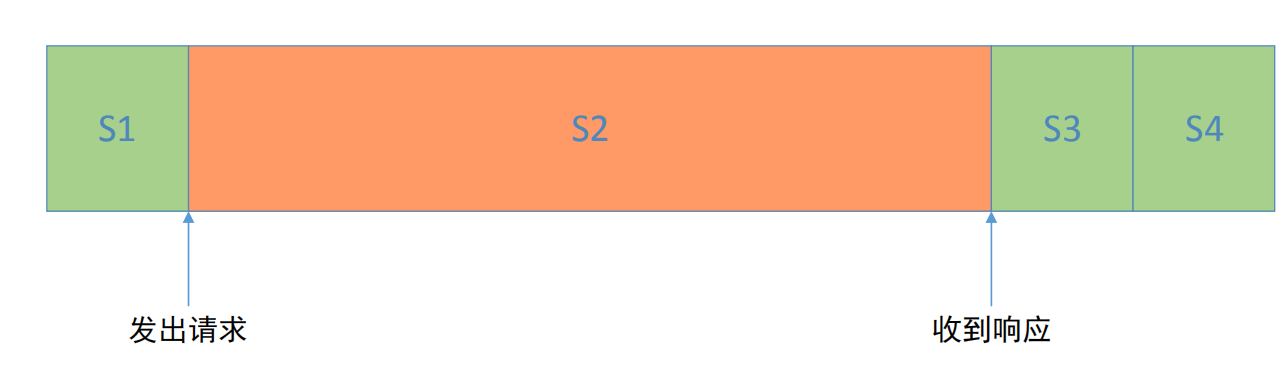
\includegraphics[width=10cm]{2.png}
\end{figure}

\subsection{进程和线程}

\textbf{进程}(Process)是计算机中的程序关于某数据集合上的一次运行活动,是系统进行资源分配和调度的基本单位,包括文本区域(text region)、数据区域(data region)和堆栈(stack region)。

比如,我们打开了一个游戏,就相当于创建了一个进程。执行这个游戏的代码(不管这个游戏是C++写的还是Java写的)就叫做这个进程的文本区域,代码运行过程中产生的变量等,会保存在数据区域,而一些临时变量,函数传递的参数等,就会放在堆栈中。

   \textbf{线程}(Thread)是被系统独立调度和分派的基本单位,是进程中执行运算的最小单位。单个进程中执行中每个任务就是一个线程,一个进程可以包含多个线程。

比如,我们打开那个游戏,这个游戏是一个进程,游戏中有匹配功能,排位功能,好友聊天功能等等,每一个功能就是一个线程。


\begin{figure}[h]
  \centering
  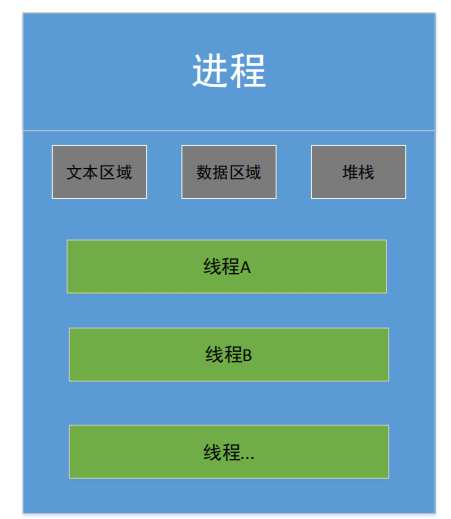
\includegraphics[width=5cm]{3.png}
\end{figure}


\subsection{多进程爬虫}

我们在打游戏的同时可以听音乐,可以看直播,并不是因为CPU同时执行这些进程,而是CPU以极短的周期交替的执行这些进程。由于进程之间切换的极快,以至于人类宏观上感觉他们是同时执行的。事实上,CPU在某一时刻只执行一个进程。

\begin{figure}[h]
  \centering
  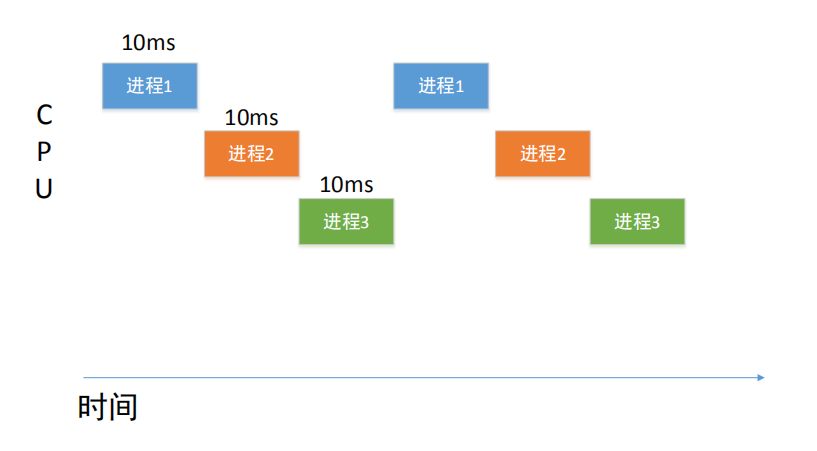
\includegraphics[width=10cm]{4.png}
\end{figure}


将每一个爬虫看成一个进程,运用多进程,如图所示

\begin{figure}[h]
  \centering
  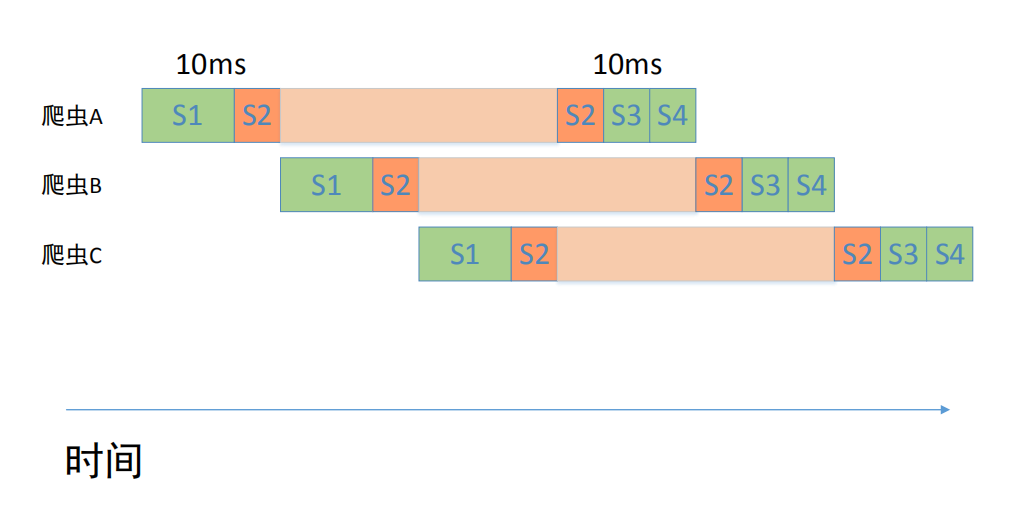
\includegraphics[width=12cm]{5.png}
\end{figure}

从图中我们可以看出,CPU首先执行爬虫$A$ 10ms,然后去执行爬虫$B$,爬虫$C$ 各10ms,当CPU返回爬虫$A$进程时,相比于上一次执行爬虫$A$已经过了20ms,所以花费更少的时间等待网站的响应内容。换句话说,CPU在一部分等待响应内容的$S2$过程中去做了别的事情。在等待爬虫$A$的响应内容时CPU完成了爬虫$B$和爬虫$C$的$S1$步骤,在等待爬虫$B$的响应内容时CPU完成了爬虫$C$的$S1$步骤和爬虫$A$的$S3$,$S4$步骤,在等待爬虫$C$的响应内容时CPU完成了爬虫$A$和爬虫$B$的$S3$,$S4$步骤。节省了总时间。


\subsection{多线程爬虫}

对于多线程爬虫,原理同多进程,只是操作系统将每个爬虫看作是一个线程,而不是一个进程。

根据计算机操作系统的相关知识,线程比进程更小,基本上不拥有系统资源,对线程之间的切换所付出的开销就会小得多。所以对于爬虫程序来说,多线程比多进程更有效。

\subsection{异步IO爬虫}



异步IO爬虫对网站发出请求后不等待返回结果,而是执行其他爬虫,等获得网页响应后再继续执行这个爬虫。如图所示



\begin{figure}[h]
  \centering
  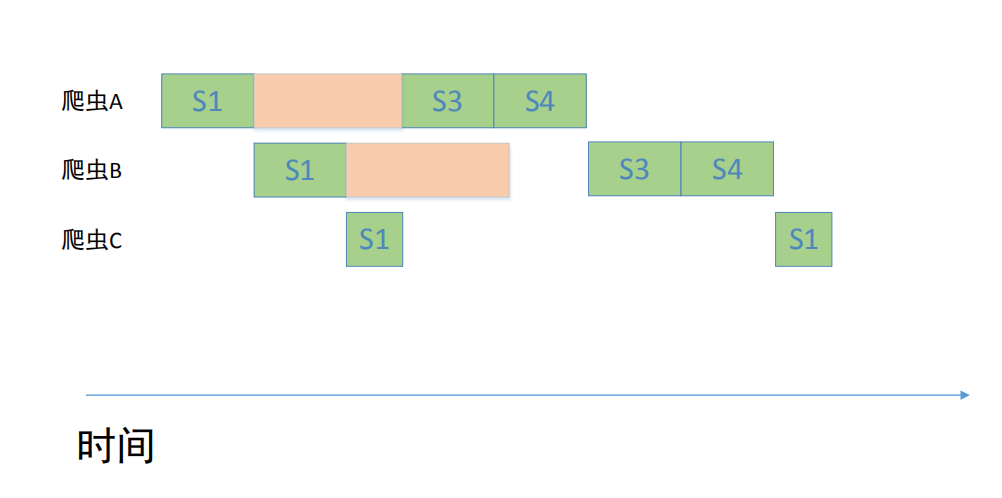
\includegraphics[width=12cm]{6.png}
\end{figure}

根据图示,异步IO利用了全部的CPU等待时间(步骤$S2$的时间),比多进程,多线程更高效


\subsection{几种爬虫的效率比较}

爬取4787个网站并将
数据存储到MySQL中
所花费的时间(3次观测)

  \begin{table}[!h]\center
\begin{tabular}{|l|l|l|l|l|}
\hline
\diagbox{次数}{爬虫类型} &普通爬虫      &     多进程爬虫  &         多线程爬虫 &      异步IO爬虫\\
\hline
第一次        &                       8分37秒         &     2分23秒   &                 59秒     &           47秒\\
\hline
第二次            &                    8分36秒         &     2分19秒   &            1分00秒       &         45秒\\
\hline
第三次            &                    8分16秒        &      2分16秒   &            1分02秒      &          48秒\\
\hline
\end{tabular}
\end{table}

可以看出,这些数据和我们上文的分析是一致的。



\section{网络爬虫实例---股票数据的获取和预测}

\subsection{股票数据的获取}

应用多线程爬虫技巧,笔者爬取了上海证券交易所和深圳证券交易所全部股票(共4627个)11天的各项数据,包括今开,昨收,最高,最低,成交量,成交额。

\begin{figure}[h]
  \centering
  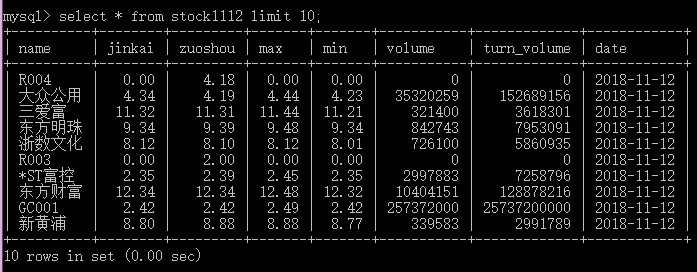
\includegraphics[width=15cm]{7.png}
\end{figure}

\subsection{股票数据的预测}

囿于笔者在股票分析方面知识的欠缺,仅用线性回归预测作为股票预测的实例,望起到抛砖引玉的效果,同时,热诚欢迎读者利用自己在股票方面的知识,更加充分地利用爬虫爬取的信息。

设股票的各项数据为$Q_{i},(i=1,2,3,4,5,6)$
将股票的各项数据看成是时间的函数$Q=f(t)$
由于在相对较短的时间内,我们可以忽略掉$f(t)$的高阶项,即将股票的数据看成是线性变化的,$Q=at+b$

根据爬虫获得的11天的信息我们可以用线性回归--最小二乘法的步骤预测股票在第12天的各项数据

Python中的sklearn库用矩阵法求解线性回归问题
矩阵法比通常代数解法要简洁,且矩阵运算可以取代循环,所以现在很多书和机器学习库都是用的矩阵法来解线性回归问题,本文将介绍这种算法。

设线性模型$$h_{\theta}(x_{1},x_{2},...,x_{n})=\theta_{0}+\theta_{1}x_{1}+\cdots+\theta_{n-1}x_{n-1}$$的矩阵表达式为$$h_{\theta}(\bm{X})=\bm{X}\theta$$
其中,假设函数$h_{\theta}(\bm{X})$为$m\times1$的向量,
$\theta$为$n\times1$的向量,$\bm{X}$为$m\times n$的矩阵,
$m$代表样本个数,$n$代表样本的特征数.

假设误差项服从高斯分布,根据线性回归的相关理论,即求损失函数$$J(\theta)=\frac{1}{2}\sum_{i=1}^{m}(h_{\theta}(x^{(i)})-y^{(i)})^{2}=\frac{1}{2}(\bm{X}\theta-\bm{Y})^{\mathrm{T}}(\bm{X}\theta-\bm{Y})$$
的最小值,其中$\bm{Y}$是样本的输出向量,维度为$m\times1$

根据最小二乘法的原理,损失函数$J(\theta)$对向量$\theta$ 的导数应该为0

\begin{align}
\frac{\partial}{\partial \theta}J(\theta)&=\frac{\partial}{\partial \theta}\left(\frac{1}{2}(\bm{X}\theta-\bm{Y})^{\mathrm{T}}(\bm{X}\theta-\bm{Y})\right)&\nonumber\\
&=\frac{\partial}{\partial \theta}\left(\frac{1}{2}((\theta^{\mathrm{T}}\bm{X}^{\mathrm{T}}-\bm{Y}))(\bm{X}\theta-\bm{Y})\right)&\nonumber\\
&=\frac{1}{2}\left(2\bm{X}^{\mathrm{T}}\bm{X}\theta-\bm{X}^{\mathrm{T}}y-(y^{\mathrm{T}}\bm{X})^{\mathrm{T}}\right)&\nonumber\\
&=\bm{X}^{\mathrm{T}}\bm{X}\theta-\bm{X}^{\mathrm{T}}y&\nonumber\\
&=0&\nonumber
\end{align}

这样即可求出$$\theta=(\bm{X}^{\mathrm{T}}\bm{X})^{-1}\bm{X}^{\mathrm{T}}y$$

通过上述算法,预测股票在第12天的各项数据

\begin{figure}[h]
  \centering
  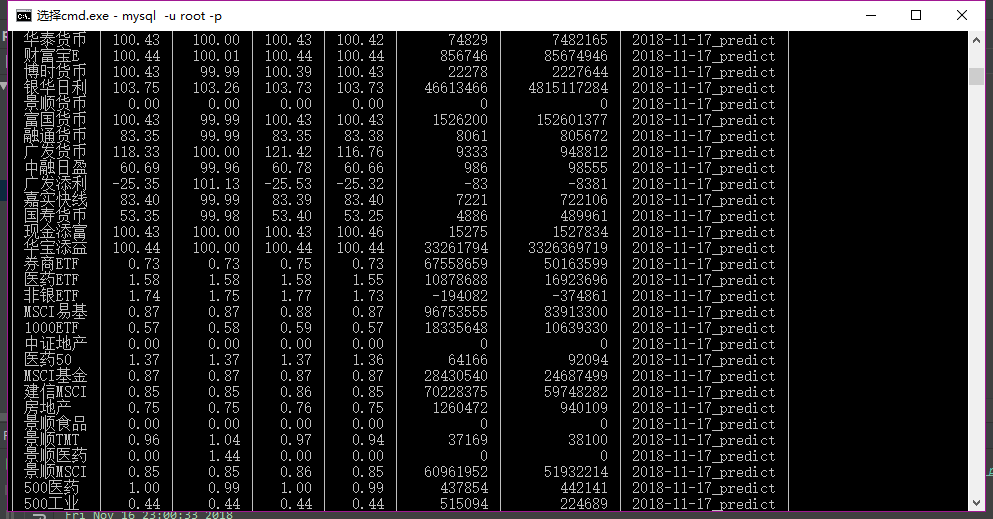
\includegraphics[width=13cm]{8.png}
\end{figure}

\section{参考文献}

[1]李俊丽. 基于Linux的python多线程爬虫程序设计[J]. 计算机与数字工程,2015,43(05):861-863+876.

[2]孙冰. 基于Python的多线程网络爬虫的设计与实现[J]. 网络安全技术与应用,2018(04):38-39.

[3]汤小丹,梁红兵,哲凤屏,汤子瀛. 计算机操作系统[M].西安:西安电子科技大学出版社, 2007.5.

[4](英)戴特. 数据库系统导论[M]. 北京:机械工业出版社,2007.

[5](挪威)赫特兰. Python基础教程[M].北京:人民邮电出版社,2010.

\section{附录}
\subsection{网络爬虫}
\begin{minted}{python}
import requests
from bs4 import BeautifulSoup
import re
import time
import pymysql


def getHTMLText(url):
    try:
        r = requests.get(url,timeout=5)
        r.raise_for_status()
        r.encoding ='gbk'
        return r.text
    except Exception as e:
        pass


def getStockList(text):
    lst=[]
    soup = BeautifulSoup(text, 'html.parser')
    a = soup.find_all('a', attrs={"target":"_blank"})
    for i in a:
        try:
            href = i.attrs['href']
            lst.append(re.findall(r"[s][hz]\d{6}", href)[0])
        except:
            continue
    return lst


def getStockData(url):
    datalist=[]
    with open('./stocklist.txt','r') as f:
        list=f.readlines()
    for s in list:
        s=s.strip('\n')
        urlnow=url+s
        k=0
        data=getHTMLText(urlnow)
        while data is None and k<10:
            data = getHTMLText(urlnow)
            k=k+1
        if k==10:
            continue
        data = data.split("=")[1]
        data = data[:-2]
        data = data.strip('\"')
        if data=="":
            continue
        print(data)
        datalist.append(data)
    return datalist


def datasaveSQL(url):
    with open('./stocklist.txt','r') as f:
        list=f.readlines()
    db = pymysql.connect("localhost", "root", "mm19990126", "test")
    cursor = db.cursor()
    for s in list:
        s=s.strip('\n')
        urlnow=url+s
        k=0
        data=getHTMLText(urlnow)
        while data is None and k<10:
            data = getHTMLText(urlnow)
            k=k+1
        if k == 10:
            continue
        data = data.split("=")[1]
        data = data[:-2]
        data = data.strip('\"')
        if data=="":
            continue
        dlist=data.split(',')
        sql = "INSERT INTO stocktest(name, jinkai, \
        zuoshou,max,min,volume,turn_volume,date) \
        VALUES ('%s', '%f', '%f', '%f','%f','%f','%f','%s' )" %
        (dlist[0],float(dlist[1]),float(dlist[2]),float(dlist[4])
        ,float(dlist[5]),float(dlist[8]),float(dlist[9]),dlist[-3])
        cursor.execute(sql)
    db.commit()
    db.close()


def savelist(lst):
    with open(r'./stocklist.txt','w') as f:
        for i in range(len(lst)):
            f.write(lst[i]+'\n')


url_list= 'http://quote.eastmoney.com/stocklist.html'
url="https://hq.sinajs.cn/list="
print(time.asctime(time.localtime(time.time())))
datasaveSQL(url)
print(time.asctime(time.localtime(time.time())))

\end{minted}

\subsection{多进程爬虫}
\begin{minted}{python}
import requests
from bs4 import BeautifulSoup
import re
import time
import pymysql
import multiprocessing


def getHTMLText(url):
    try:
        r = requests.get(url,timeout=5)
        r.raise_for_status()
        r.encoding ='gbk'
        return r.text
    except Exception as e:
        pass


def getStockList(text):
    lst=[]
    soup = BeautifulSoup(text, 'html.parser')
    a = soup.find_all('a', attrs={"target":"_blank"})
    for i in a:
        try:
            href = i.attrs['href']
            lst.append(re.findall(r"[s][hz]\d{6}", href)[0])
        except:
            continue
    return lst


def getStockData(url):
    datalist=[]
    with open('./stocklist.txt','r') as f:
        list=f.readlines()
    for s in list:
        s=s.strip('\n')
        urlnow=url+s
        k=0
        data=getHTMLText(urlnow)
        while data is None and k<10:
            data = getHTMLText(urlnow)
            k=k+1
        if k==10:
            continue
        data = data.split("=")[1]
        data = data[:-2]
        data = data.strip('\"')
        if data=="":
            continue
        datalist.append(data)
    return datalist


def datafind(url,s):              #for multiprocess
    s=s.strip('\n')
    urlnow=url+s
    k=0
    data=getHTMLText(urlnow)
    while data is None and k<10:
        data = getHTMLText(urlnow)
        k=k+1
    if k==10:
        data= []
    else:
        data = data.split("=")[1]
        data = data[:-2]
        data = data.strip('\"')
        data=data.split(',')
    return data


def singleinsert(data):              #for multiprocess
    if data!=['']:
        dlist = data
        sql = "INSERT INTO stock1106(name, jinkai, zuoshou\
        ,max,min,volume,turn_volume,date) \
                VALUES ('%s', '%f', '%f', '%f','%f','%f','%f','%s' )" % (
        dlist[0], float(dlist[1]), float(dlist[2]), float(dlist[4]),
        float(dlist[5]), float(dlist[8]), float(dlist[9]),
        dlist[-3])
        cursor.execute(sql)


if __name__ == '__main__':

    print(time.asctime(time.localtime(time.time())))

    url = "https://hq.sinajs.cn/list="
    with open(r'./stocklist.txt', 'r') as f:
        slist = f.readlines()
    db = pymysql.connect("localhost", "root", "mm19990126", "test")
    cursor = db.cursor()
    pool = multiprocessing.Pool()
    for s in slist:
        pool.apply_async(datafind,args=(url,s,), callback=singleinsert)
    pool.close()
    pool.join()
    db.commit()
    db.close()
    print(time.asctime(time.localtime(time.time())))

\end{minted}
\subsection{多线程爬虫}
\begin{minted}{python}
import requests
from bs4 import BeautifulSoup
import re
import time
import pymysql
import threadpool
import threading


def getHTMLText(url):
    try:
        r = requests.get(url,timeout=5)
        r.raise_for_status()
        r.encoding ='gbk'
        return r.text
    except Exception as e:
        pass


def getStockList(text):
    lst=[]
    soup = BeautifulSoup(text, 'html.parser')
    a = soup.find_all('a', attrs={"target":"_blank"})
    for i in a:
        try:
            href = i.attrs['href']
            lst.append(re.findall(r"[s][hz]\d{6}", href)[0])
        except:
            continue
    return lst


def getStockData(url):
    datalist=[]
    with open('./stocklist.txt','r') as f:
        list=f.readlines()
    for s in list:
        s=s.strip('\n')
        urlnow=url+s
        k=0
        data=getHTMLText(urlnow)
        while(data==None and k<10):
            data = getHTMLText(urlnow)
            k=k+1
        if k==10:
            continue
        data = data.split("=")[1]
        data = data[:-2]
        data = data.strip('\"')
        if data=="":
            continue
        datalist.append(data)
    return datalist


def datafind(s):                          #for multithread
    url = "https://hq.sinajs.cn/list="
    s=s.strip('\n')
    urlnow=url+s
    k=0
    data=getHTMLText(urlnow)
    while(data==None and k<10):
        data = getHTMLText(urlnow)
        k=k+1
    if k==10:
        data= []
    else:
        data = data.split("=")[1]
        data = data[:-2]
        data = data.strip('\"')
        data=data.split(',')
    return data


def singleinsert(data):                       #for multithread
    if data!=['']:
        dlist = data
        sql = "INSERT INTO stock1116(name, jinkai, zuoshou,\
        max,min,volume,turn_volume,date) \
                VALUES ('%s', '%f', '%f', '%f','%f','%f','%f','%s' )" % (
        dlist[0], float(dlist[1]), float(dlist[2]), float(dlist[4]),
        float(dlist[5]), float(dlist[8]), float(dlist[9]),dlist[-3])
        cursor.execute(sql)


def whole(s):
    data=datafind(s)
    if mutex.acquire(True):
        singleinsert(data)
        mutex.release()


if __name__ == '__main__':

    print(time.asctime(time.localtime(time.time())))
    mutex = threading.Lock()
    url = "https://hq.sinajs.cn/list="
    with open(r'./stocklist.txt', 'r') as f:
        slist = f.readlines()
    db = pymysql.connect("localhost", "root", "mm19990126", "test")
    cursor = db.cursor()

    threads = []
    for s in slist:
        t = threading.Thread(target=whole, args=(s,))
        threads.append(t)
    for t in threads:
        t.start()
    for t in threads:
        t.join()
    db.commit()
    db.close()
    print(time.asctime(time.localtime(time.time())))

\end{minted}

\subsection{异步IO爬虫}
\begin{minted}{python}
import asyncio
import aiohttp
import pymysql
import time


async def getpage(s):
    try:
        url = "https://hq.sinajs.cn/list="
        s = s.strip('\n')
        urlnow=url+s
        async with aiohttp.request('GET',urlnow) as r:
            res = await r.text(encoding='gbk')
        data=res
        k=0
        while data==None and k<10:
            async with aiohttp.request('GET', urlnow) as r:
                res = await r.text(encoding='gbk')
            data = res
        data = data.split("=")[1]
        if data!="":
            data = data[:-2]
            data = data.strip('\"')
            data = data.split(',')
            singleinsert(data)
    except:
        pass


def singleinsert(data):
    if data!=['']:
        dlist = data
        sql = "INSERT INTO stocktest2(name, jinkai, zuoshou,\
        max,min,volume,turn_volume,date) \
        VALUES ('%s', '%f', '%f', '%f','%f','%f','%f','%s' )" % (
        dlist[0], float(dlist[1]), float(dlist[2]), float(dlist[4]),
        float(dlist[5]), float(dlist[8]), float(dlist[9]),dlist[-3])
        cursor.execute(sql)


def runEventLoop():
    loop = asyncio.new_event_loop()
    asyncio.set_event_loop(loop)
    loop.run_until_complete(getpage(s))
    loop.close()


if __name__=='__main__':
    print(time.asctime(time.localtime(time.time())))
    tasks = []
    with open(r'./stocklist.txt', 'r') as f:
        slist = f.readlines()
    db = pymysql.connect("localhost", "root", "mm19990126", "test")
    cursor = db.cursor()
    for s in slist[0:499]:
        tasks.append(asyncio.ensure_future(getpage(s)))
    loop = asyncio.get_event_loop()
    loop.run_until_complete(asyncio.wait(tasks))
    loop.close()
    tasks = []
    db.commit()
    db.close()
    print(time.asctime(time.localtime(time.time())))
\end{minted}
\subsection{股票的预测}
\begin{minted}{python}
import pymysql
from sklearn import linear_model
import numpy
import time


def datasearch(code,cursor):

    sql="SELECT * FROM test WHERE code='%s';" % (code)
    cursor.execute(sql)
    name=cursor.fetchone()
    if name==None:
        return []
    name=name[0]
    data=[]
    for i in stockdate:
        sqlsearch="SELECT * FROM %s WHERE name='%s';" % (i,name)
        cursor.execute(sqlsearch)
        data.append(cursor.fetchone())
    if len(data)<11:
        data=[]

    return data


def linear_model_main(Xlist, Ylist):
    regr = linear_model.LinearRegression()
    regr.fit(Xlist, Ylist)
    return regr.coef_, regr.intercept_


def predict(data):
    outcome=[]
    outcome.append(data[0][0])
    for i in range(1,7):
        y=[]
        for s in range(len(stockdate)):
            y.append(float(data[s][i]))
        y1=numpy.array(y)
        intarray=numpy.array(intdate)
        a,b=linear_model_main(intarray.reshape(-1,1),y1.reshape(-1,1))
        pre1=a*17+b
        pre1=float(pre1)
        outcome.append(pre1)
    outcome.append('2018-11-17_predict')
    return outcome


def singleinsert(data,cursor):
    dlist = data
    sql = "INSERT INTO stockpredict(name, jinkai, zuoshou,\
    max,min,volume,turn_volume,date) \
    VALUES ('%s', '%.2f', '%.2f', '%.2f','%.2f','%.2f','%.2f','%s' )" % (
    dlist[0], float(dlist[1]), float(dlist[2]), float(dlist[3]),
    float(dlist[4]), float(dlist[5]), float(dlist[6]),dlist[7])
    cursor.execute(sql)


def whole(code,cursor):
    try:
        data=datasearch(code,cursor)
        if data==[]:
            return ''
        outcome=predict(data)
        singleinsert(outcome,cursor)
    except:
        pass


print(time.asctime(time.localtime(time.time())))
date = ['02', '05', '06', '07', '08', '09', '12', '13', '14', '15', '16']
stockdate=[]
intdate=[]
for i in date:
    stockdate.append('stock11'+i)
    intdate.append(int(i))
with open(r'./stocklist.txt', 'r') as f:
    slist = f.readlines()
db = pymysql.connect("localhost", "root", "mm19990126", "test")
cursor = db.cursor()
for s in slist:
    i = s.strip('\n')
    whole(i,cursor)
db.commit()
db.close()
print(time.asctime(time.localtime(time.time())))
\end{minted}
\end{document}
